\documentclass[a4paper,12pt]{article}
\usepackage{amsmath,amssymb,amsfonts,amsthm, bpchem}
\usepackage{tikz}
\usepackage [utf8x] {inputenc}
\usepackage [T2A] {fontenc} 
\usepackage[russian]{babel}
\usepackage{cmap} 
\usepackage{ gensymb }
\usepackage[unicode]{hyperref}
\usepackage{ textcomp }
\usepackage{indentfirst} 


\usepackage{graphicx}

\usepackage[margin=1in]{geometry}


\usepackage{fancyhdr}
\usepackage{wrapfig}

\newcommand{\bbR}{\mathbb R}
\newcommand{\eps}{\varepsilon}
\newcommand{\bbN}{\mathbb N}
\newcommand{\dif}{\mathrm{d}}

\newtheorem{Def}{Определение}


\pagestyle{fancy}
\makeatletter 
\fancyhead[L]{\footnotesize  MolVision}
\fancyhead[R]{\footnotesize  Проект}
\fancyfoot[R]{\thepage}
\fancyfoot[C]{}

\renewcommand{\maketitle}{%
	\noindent{\bfseries\scshape\large\@title\ \mdseries\upshape}\par
	\noindent {\large\itshape\@author}
	\vskip 2ex}
\makeatother
\def\dd#1#2{\frac{\partial#1}{\partial#2}}

\begin{document}

\renewcommand{\figurename}{\textbf{Рис.}}		
\renewcommand{\tablename}{\textbf{Таблица}}	


\begin{titlepage}
	\centering
	
\includegraphics[width=0.4\textwidth]{DBMP.png}\par\vspace{2 cm}
	{\scshape\LARGE\itshape Московский физико-технический институт \par}
	\vspace{1cm}
	{\scshape\LARGE\itshape Факультет биологической и медицинской физики \par}
	\vspace{0.5cm}
	{\scshape\Large  Проект по курсу информатики (Python 3) \par}
	\vspace{1.5cm}
	{\huge\bfseries Визуализация и работа с химическими молекулами \par}
	{\huge\bfseries "MolVision" \par}
	\vspace{2cm}
	{\Large\itshape Выполнила Щербина Елизавета Николаевна \par}
	{\Large\itshape Группа 6115 \par}
	%\vfill
	%supervised by\par
	%Dr.~Mark \textsc{Brown}
	
	%\vfill
	
	% Bottom of the page
	{\large 4 учебный семестр\par}
\end{titlepage}

\newpage
\section{Введение}
\paragraph{} \textbf{Химия} - это одна из основных наук естествознания, изучающая внутренний состав, внутреннее строение материи, закономерности качественных изменений, разложения и превращения веществ, а также закономерности образования новых веществ в результате качественных изменений.
\paragraph{} Именно благодаря достижениям в этой науке человечество стремительно продолжает развиваться. С помощью неё мы не перестаем бороться с самыми страшными заболеваниями, получаем возможность сохранить и обезопасить урожай от вредителей или улучшить плодородие земли. Сложно представить, насколько химия глубоко внедрена в нашу жизнь.
\paragraph{} На протяжении последних десятилетий химия развивается наиболее стремительно, ей занимаются в самых разных местах нашей планеты.

\section{Актуальность проблемы}
\paragraph{} Из-за того, что многие лаборатории занимаются развитием химии независимо друг от друга, возникают проблемы, решение которых совсем не тривиально. 
\paragraph{} Самые актуальные из них - проблемы с спецификацией (системой правил однозначного описания состава и структуры молекулы химического вещества): группы придумывают свои варианты зашифровывания структур молекул, что не может не вызывать вопросов при кооперации между деятельными лабораториями. На данный момент существует более 50 различных спецификаций, самые популярные из которых SMILES, sdf, pdb, mol.

\section{Цель проекта и суть}
\paragraph{} Целью данного проекта является возможность визуализировать молекулы. Увидеть, как выглядит тот или иной объект, оценить возможное взаимодействие между атомами, их геометрию. Модель строится в 3D формате и позволяет посмотреть на неё со всех сторон. 

\subsection{Почему SMILES}
\paragraph{} \textbf{SMILES} - Simplified Molecular Input Line Entry System, с англ. — «система упрощённого представления молекул в строке ввода». Это одна из самых распространенных в мире спецификаций, генерация которой имеет интересный смысл.
\paragraph{} В терминах теории графов SMILES представляет собой строку, полученную путём вывода символов вершин молекулярного графа в порядке, соответствующем их обходу в глубину. Первоначальная обработка графа включает в себя удаление атомов водорода и разбивку циклов таким образом, чтобы получившийся граф представлял собой остовный лес. Местам разбиения графа ставятся в соответствие числа, показывающие наличие связи в исходной молекуле. Для указания точек ветвления молекулы используются скобки.
\paragraph{} Формула SMILES может быть преобразована в двухмерную структурную формулу при помощи алгоритма (Structure Diagram Generation algorithms), разработанного Хелсоном. Преобразование не всегда даёт однозначный результат. Преобразование в трехмерную структурную формулу производится с использованием принципа минимальной энергии образования вещества.

\subsection{Действие}
\begin{itemize}
\item Программа предлагает ввести нужную молекулу в формате SMILES
\item Выводит её координаты в терминал 
\item Рисует в новом окне 3D-структуру молекулы
\end{itemize}

\section{Пример}
В качестве примера нарисуем молекулу пирокатехина (SMILES: Oc1ccccc1O), имеющую следующий вид:

\begin{center}
    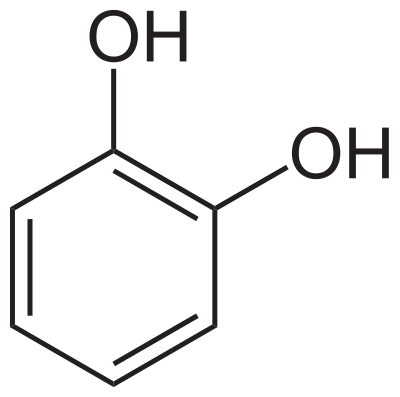
\includegraphics[width=0.2\textwidth]{Pirocatechin.png}\par\vspace{1 cm}
\end{center} 


\paragraph{} Запускаем программу:

\begin{center}
    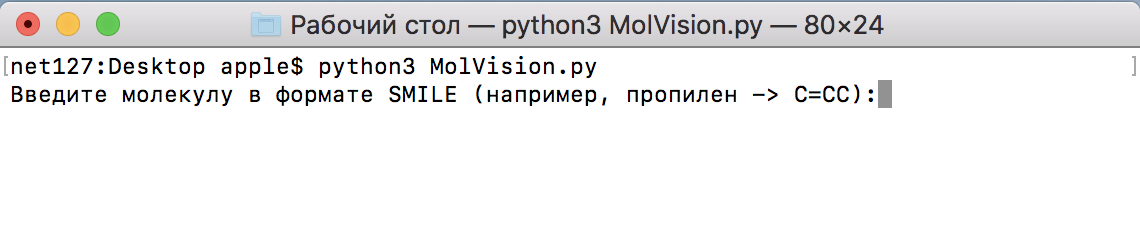
\includegraphics[width=1\textwidth]{enter.png}\par\vspace{1 cm}
\end{center} 

\paragraph{} Вводим молекулу пирокатехина и получаем нужные для построения координаты:
\begin{center}
    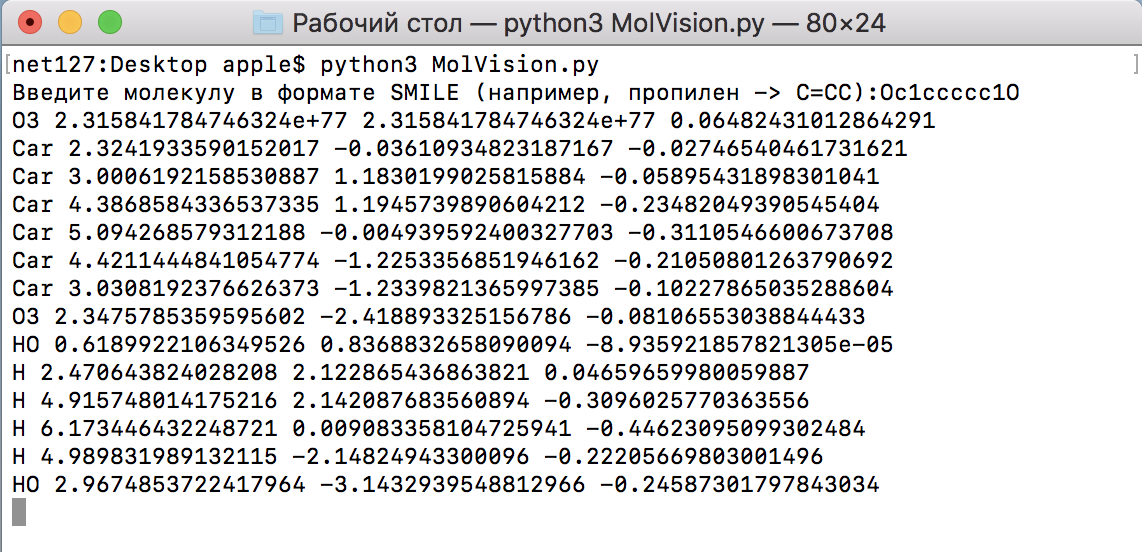
\includegraphics[width=1\textwidth]{table.png}\par\vspace{1 cm}
\end{center} 

\paragraph{} Наша полученная модель молекулы:
\begin{center}
    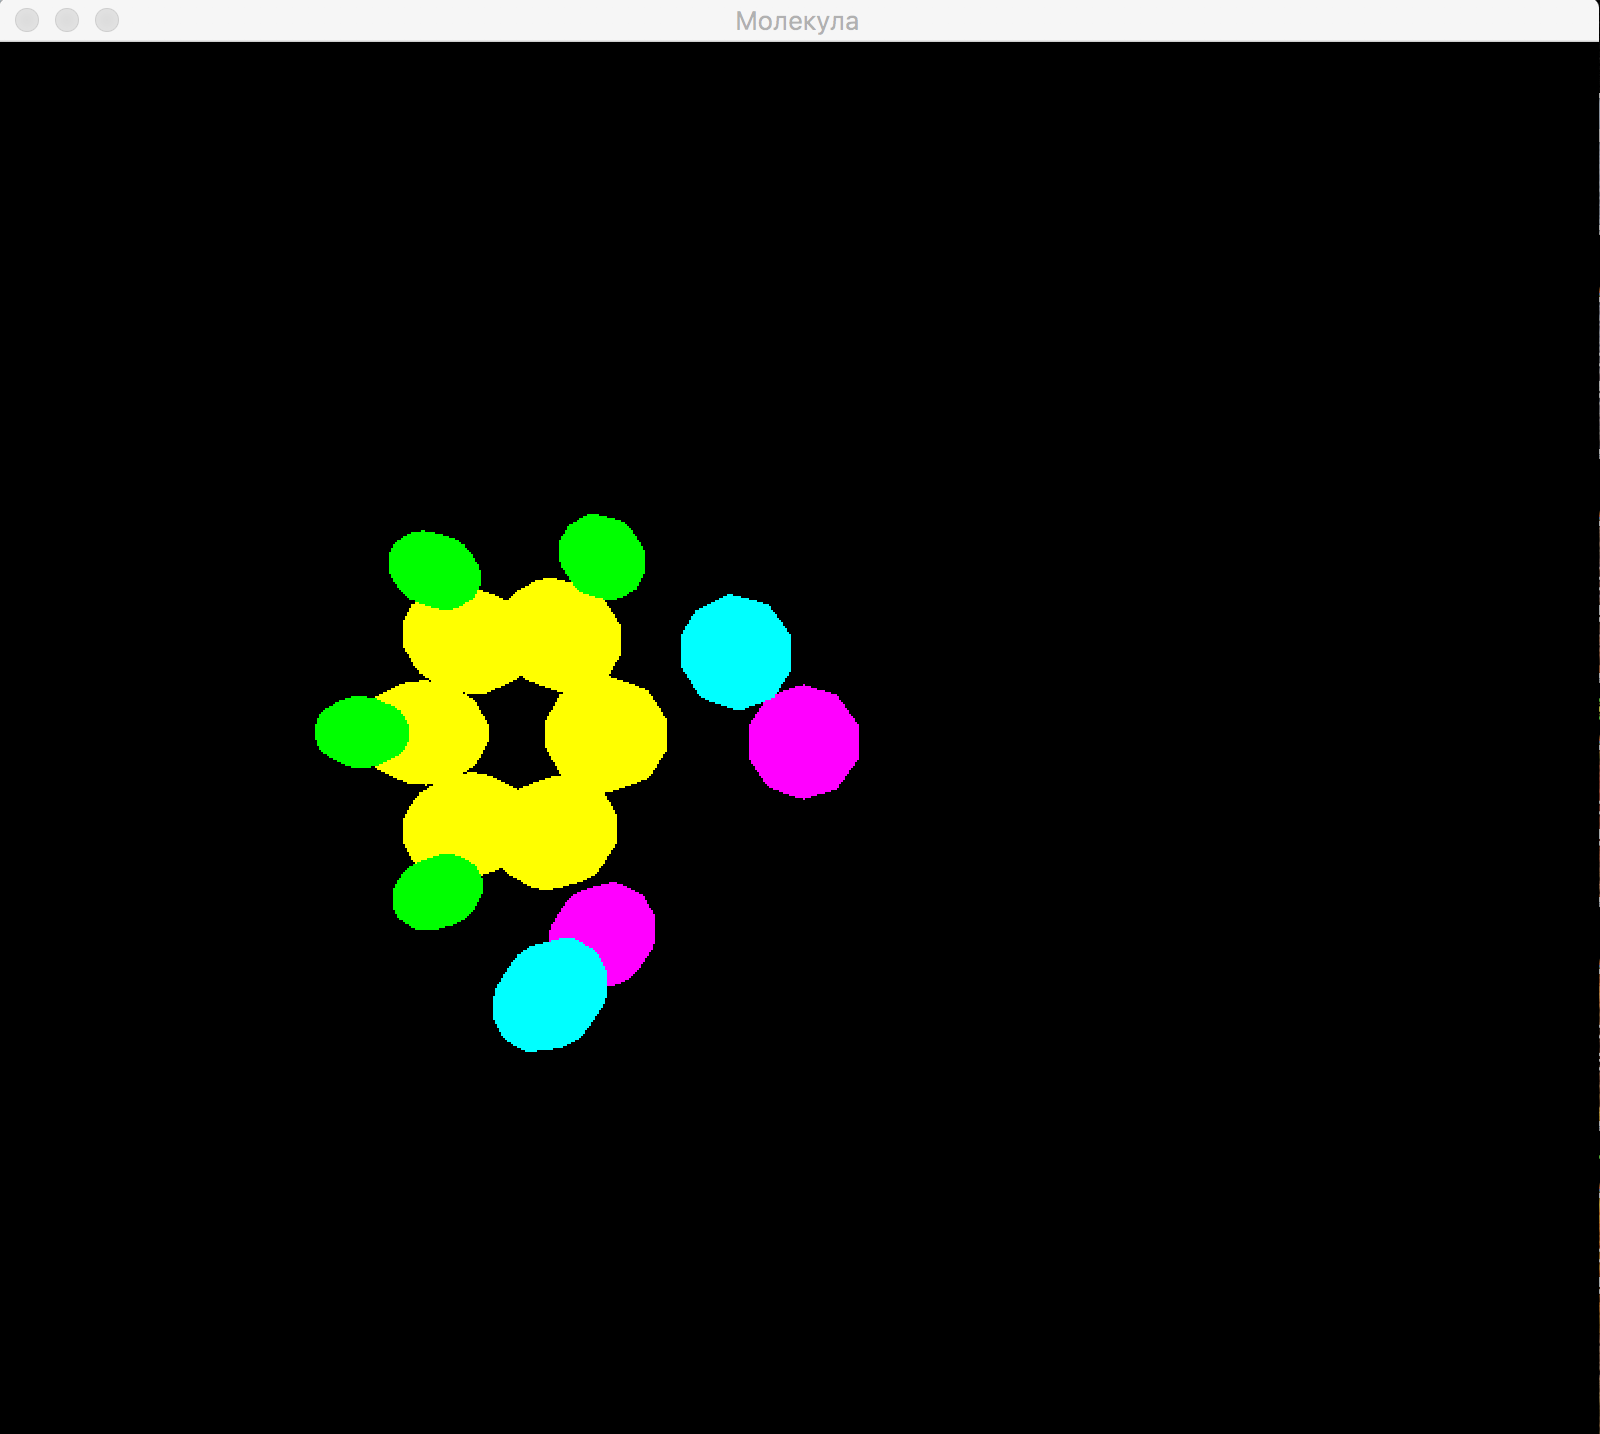
\includegraphics[width=0.9\textwidth]{molecule.png}\par\vspace{1 cm}
\end{center} 

\section{Обсуждение и вывод}
\paragraph{} В ходе данной работы мы научились работать с классами молекул, рисовать объекты с помощью известной и многофункциональной библиотеки OpenGL, познакомились с методами работы в OpenBabel (Pybel - её составляющая), вспомнили работу с двумерными массивами, особенности Python3. 
\paragraph{} Также с помощью этой программы можно загружать файл полностью, без ввода. Можно поменять формат ввода и дополнить его.
\paragraph{} Здесь приблизительно сохранены размеры молекул, группы одинаковых молекул раскрашены одним цветом, что позволяет сделать выводы о геометрии и возможных активных частей молекул. 
\paragraph{} Данная работа лишь начало более серьёзной программы для хемоинформатики, работы с разными спецификациями, считывании и визуализации молекул. Поле для разработки ещё очень большое.

\section{Использованные библиотеки}
\paragraph{} В ходе данной работы были использованы несколько дополнительных библиотек:
\begin{itemize}
\item Pygame
\item OpenGL
\item Pybel
\end{itemize}

\end{document}
